\chapter{Dataset and Data Preprocessing}

\section{LISA Traffic Light Dataset}

The LISA Traffic Light Dataset is a publicly available resource for traffic light detection research. The version used in this project was obtained via the Data Ninja platform in Supervisely JSON format, comprising 20,535 training images and 22,481 test images at a resolution of 1280$\times$960 pixels. The images represent sequential video frames captured from a forward-facing dashcam mounted in a moving vehicle, covering both daytime (14,034 frames) and night-time (6,501 frames) conditions across multiple US traffic scenarios.

\section{Annotation Format}

Each image in the dataset is accompanied by a corresponding JSON annotation file. Annotations describe the spatial location of each traffic light as a bounding box defined by two corner coordinates, along with a class label denoting the light's state. The dataset originally contains 14 distinct class labels reflecting directional variants of each state (e.g., ``go left traffic light'', ``stop traffic light'', ``warning left''). The annotation files follow the Supervisely format, where each object entry contains a class title and the exterior corner coordinates of the bounding rectangle.

Figure~\ref{fig:train_batch} illustrates sample annotated training images.

\begin{figure}[ht]
    \begin{center}
        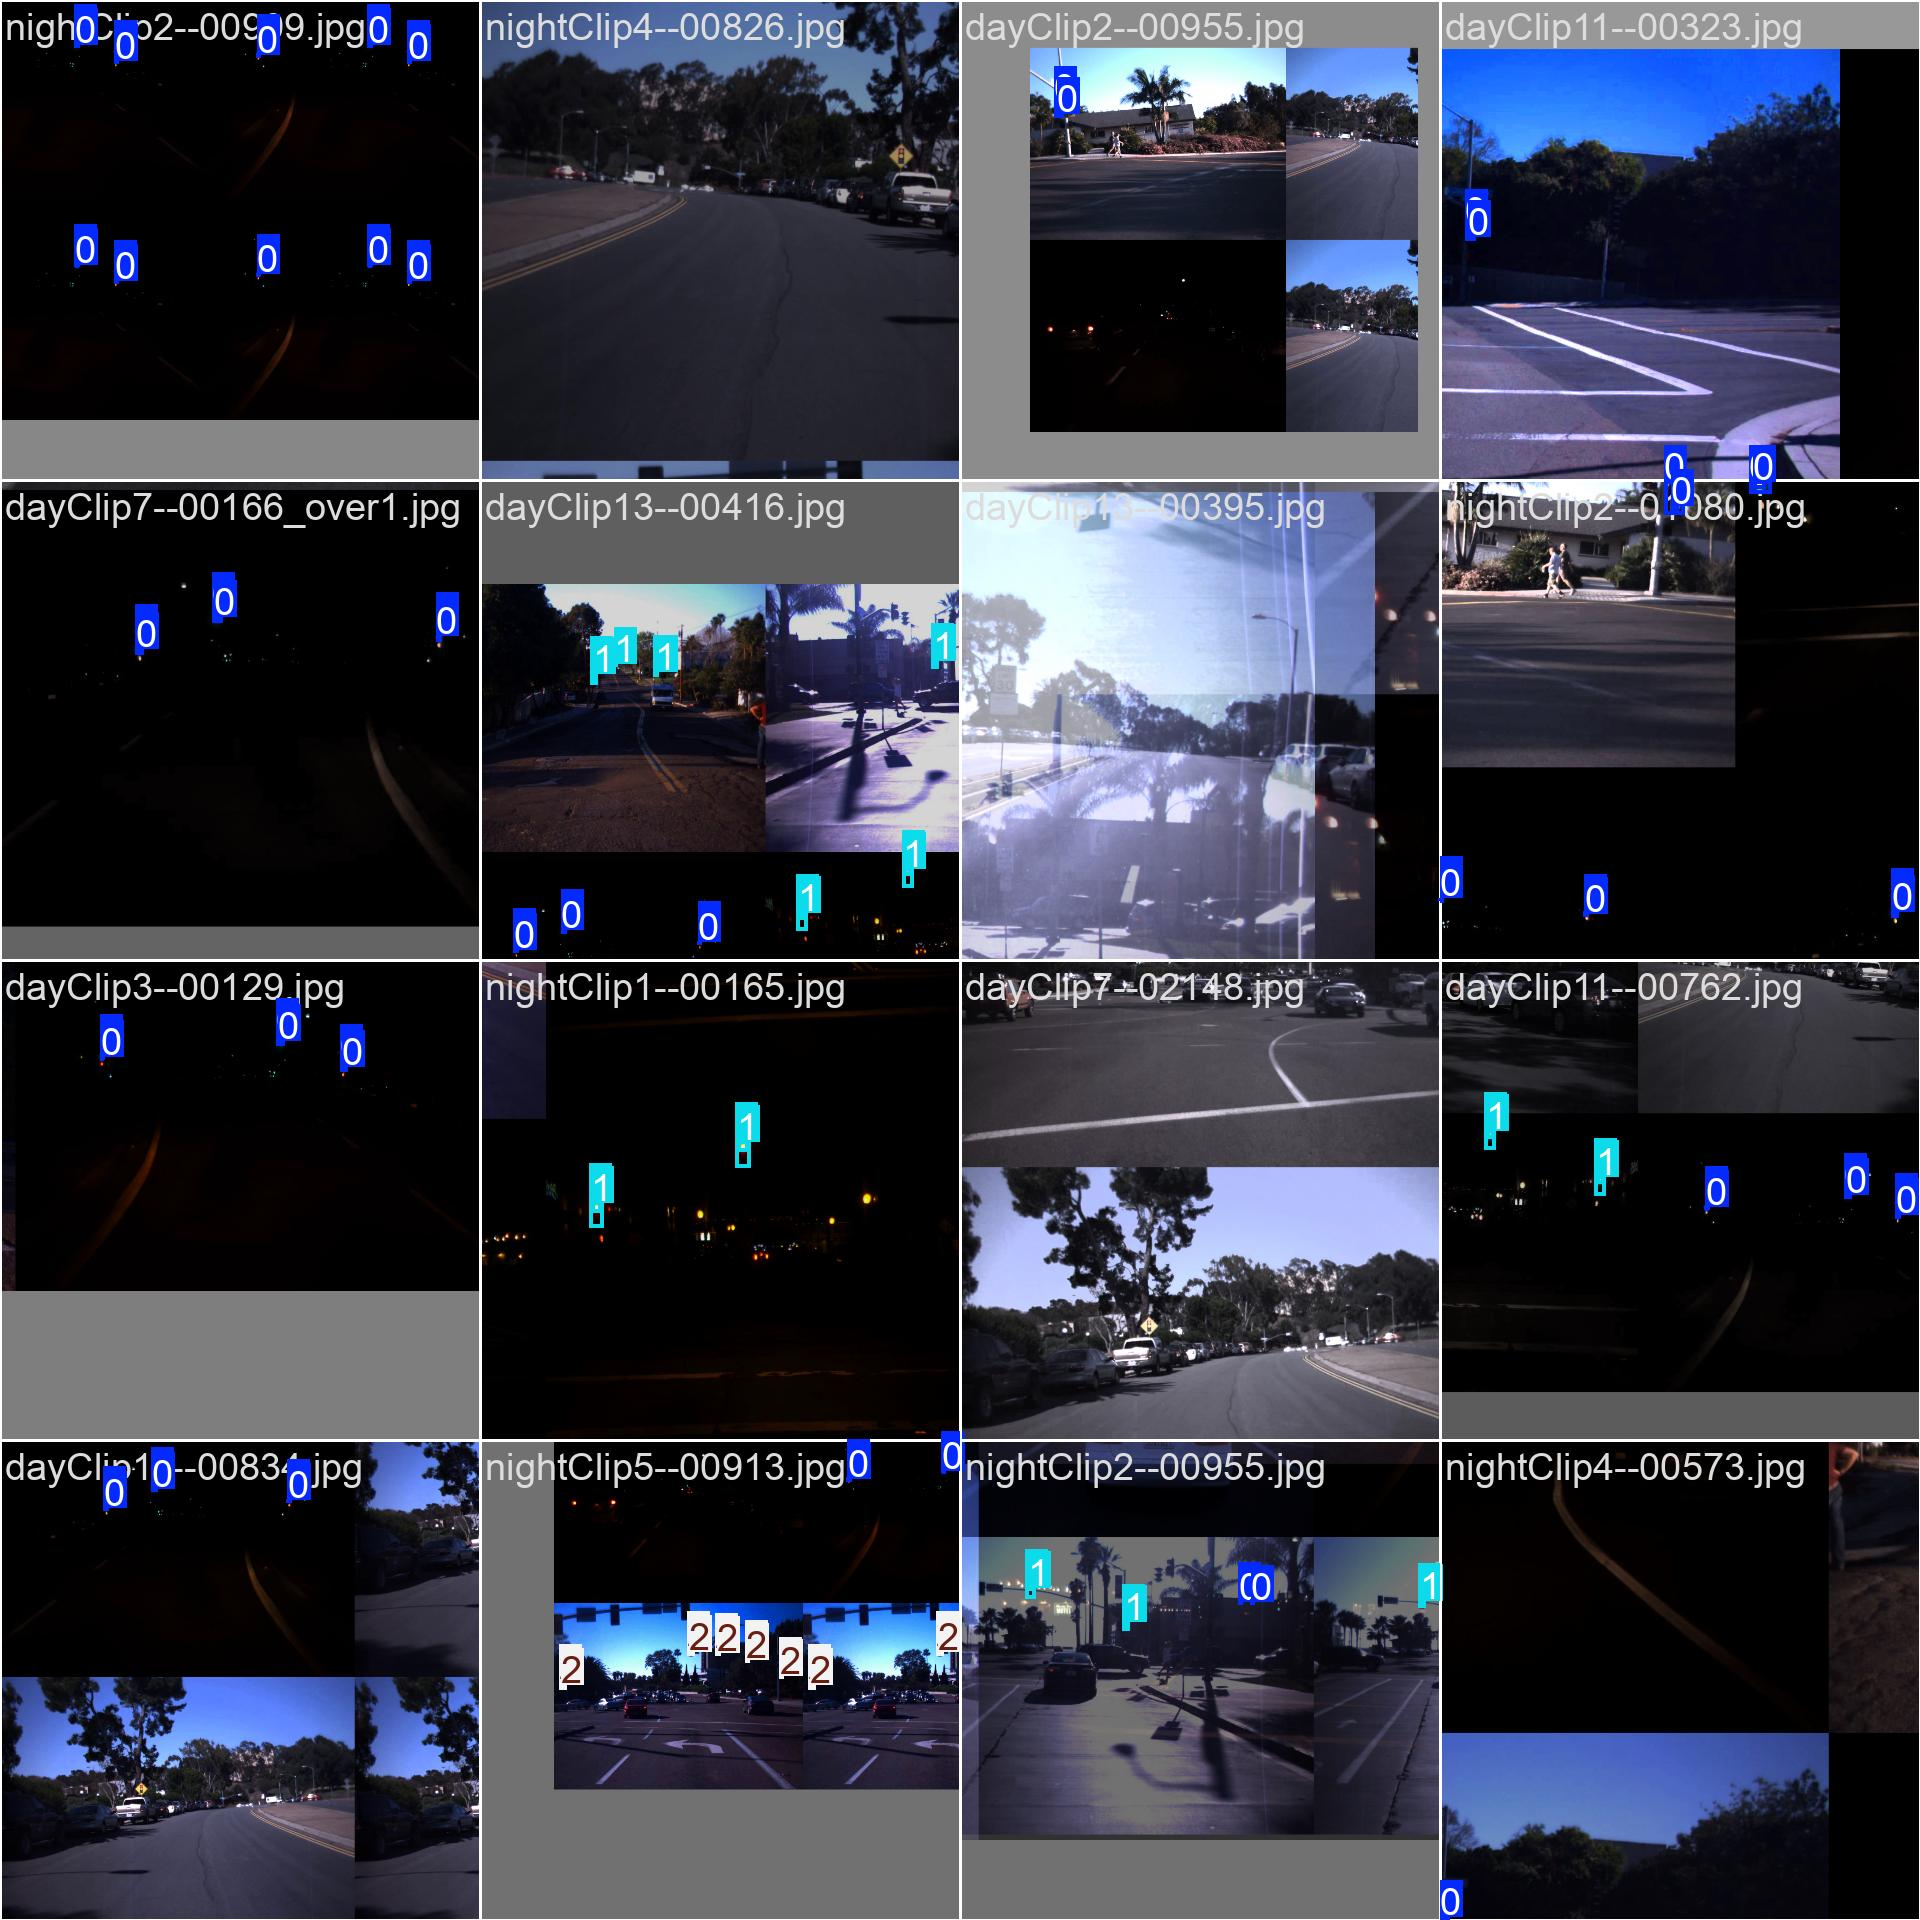
\includegraphics[width=\textwidth]{Images/Chapter2/train_batch0.jpg}
    \end{center}
    \caption{Sample annotated training images showing traffic light bounding boxes.}
    \label{fig:train_batch}
\end{figure}

\section{Exploratory Data Analysis}

\subsection{Class Distribution}\label{sec:eda-class-dist}

Prior to preprocessing, a statistical analysis of the annotation data was conducted to understand class frequencies. The dataset contains approximately 219,832 annotated bounding boxes in the training split. Following the mapping of 14 raw classes to three semantic categories, the distribution is highly imbalanced: the stop class accounts for approximately 114,000 instances (52\%), the go class for approximately 99,000 instances (45\%), and the warning class for only approximately 6,000 instances (2.8\%). This represents a 19:1 ratio between the most and least frequent classes, as shown in Figure~\ref{fig:class_dist}. Such imbalance, if left uncorrected, would result in a model biased toward the dominant classes with poor sensitivity to warning lights.

\begin{figure}[ht]
    \begin{center}
        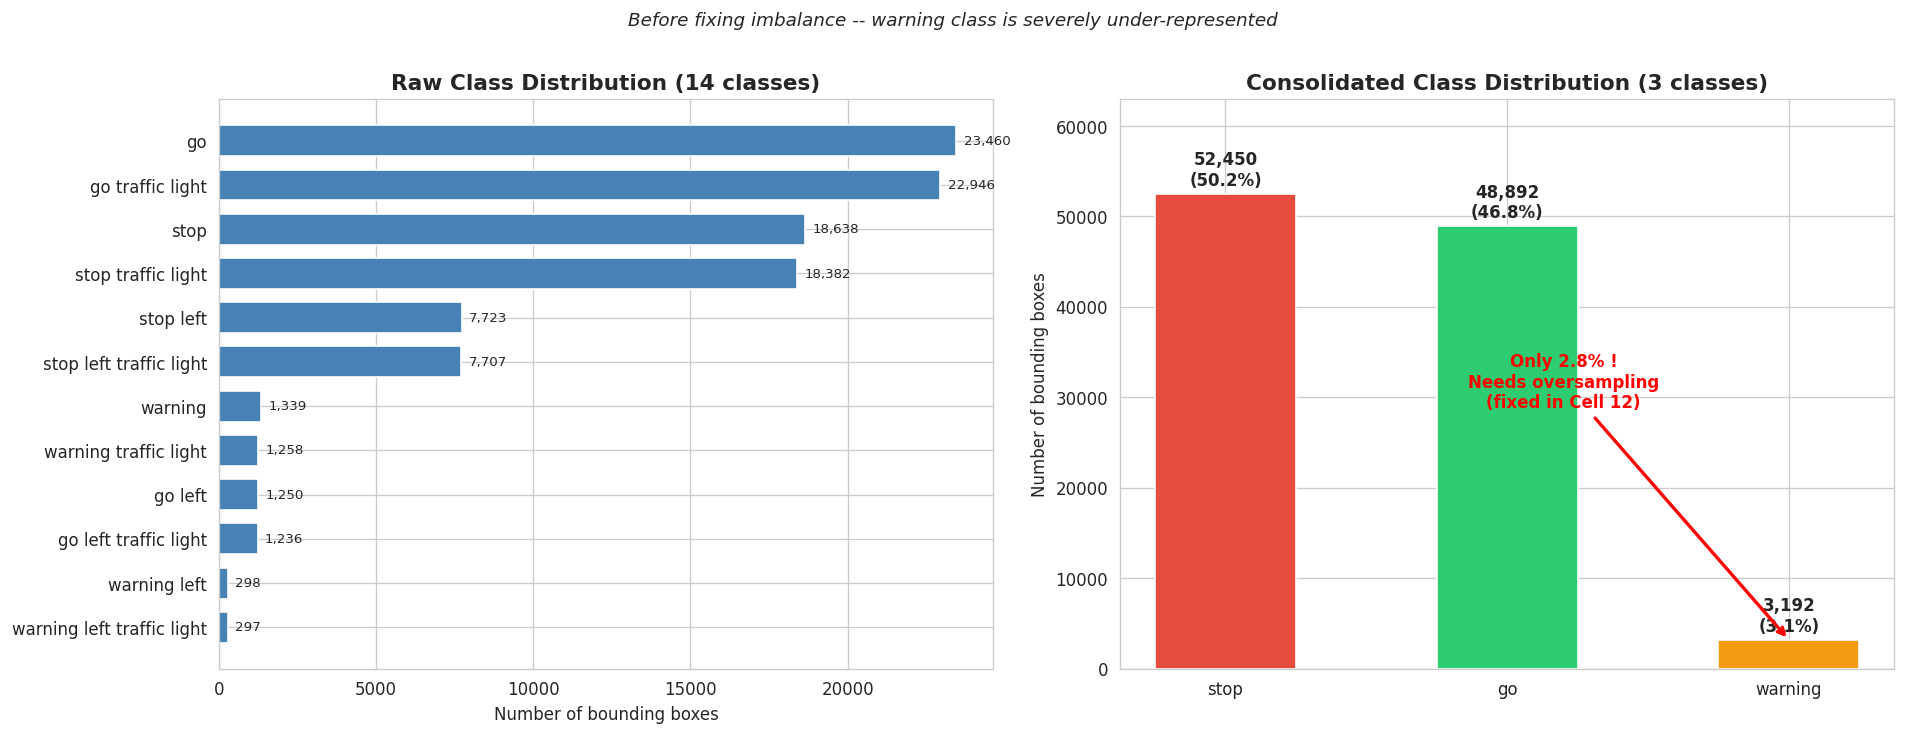
\includegraphics[width=0.85\textwidth]{Images/Chapter2/class_distribution.png}
    \end{center}
    \caption{Class distribution of annotated instances in the training split, showing severe imbalance between stop, go, and warning classes.}
    \label{fig:class_dist}
\end{figure}

\subsection{Bounding Box Size Analysis}

An analysis of bounding box dimensions revealed that traffic lights in this dataset are predominantly small objects. The mean bounding box measures approximately 20$\times$33 pixels on a 1280$\times$960 image, corresponding to just 0.05\% of the total image area. Classifying boxes according to the COCO benchmark size categories (Tiny: height $<$ 20\,px, Small: 20--32\,px, Medium: 32--96\,px, Large: $>$96\,px), approximately 96\% of annotated instances fall into the Tiny or Small categories, as illustrated in Figure~\ref{fig:bbox}. This finding has two key implications: (1) the input resolution must be kept high (1280 pixels) to preserve detail in small objects, and (2) a model with a deep feature pyramid (YOLOv8s) is preferred over a lighter model (YOLOv8n) to detect fine-grained features at multiple scales.

\begin{figure}[ht]
    \begin{center}
        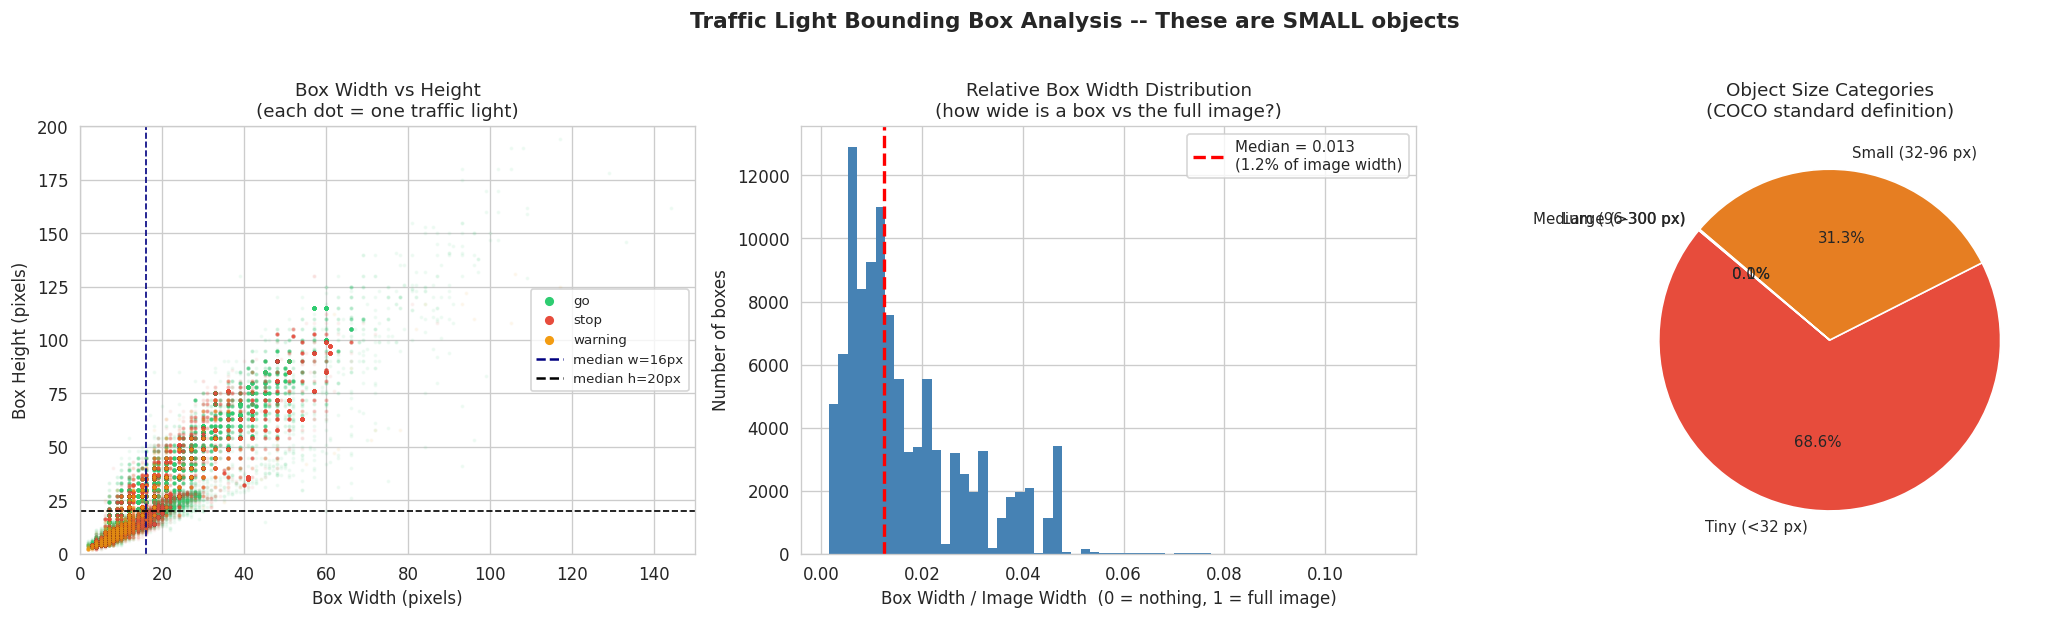
\includegraphics[width=\textwidth]{Images/Chapter2/bbox_analysis.png}
    \end{center}
    \caption{Bounding box size analysis showing the distribution of traffic light dimensions. The majority of instances fall in the Tiny and Small size categories.}
    \label{fig:bbox}
\end{figure}

\subsection{Sample Images Per Class}

Figure~\ref{fig:class_samples} presents representative samples from each of the three semantic classes with their corresponding bounding box annotations. Green-bordered boxes indicate go lights, red-bordered boxes indicate stop lights, and orange-bordered boxes indicate warning lights. The visualisation confirms correct class assignment and illustrates the variation in lighting conditions, light size, and scene context present in the dataset.

\begin{figure}[ht]
    \begin{center}
        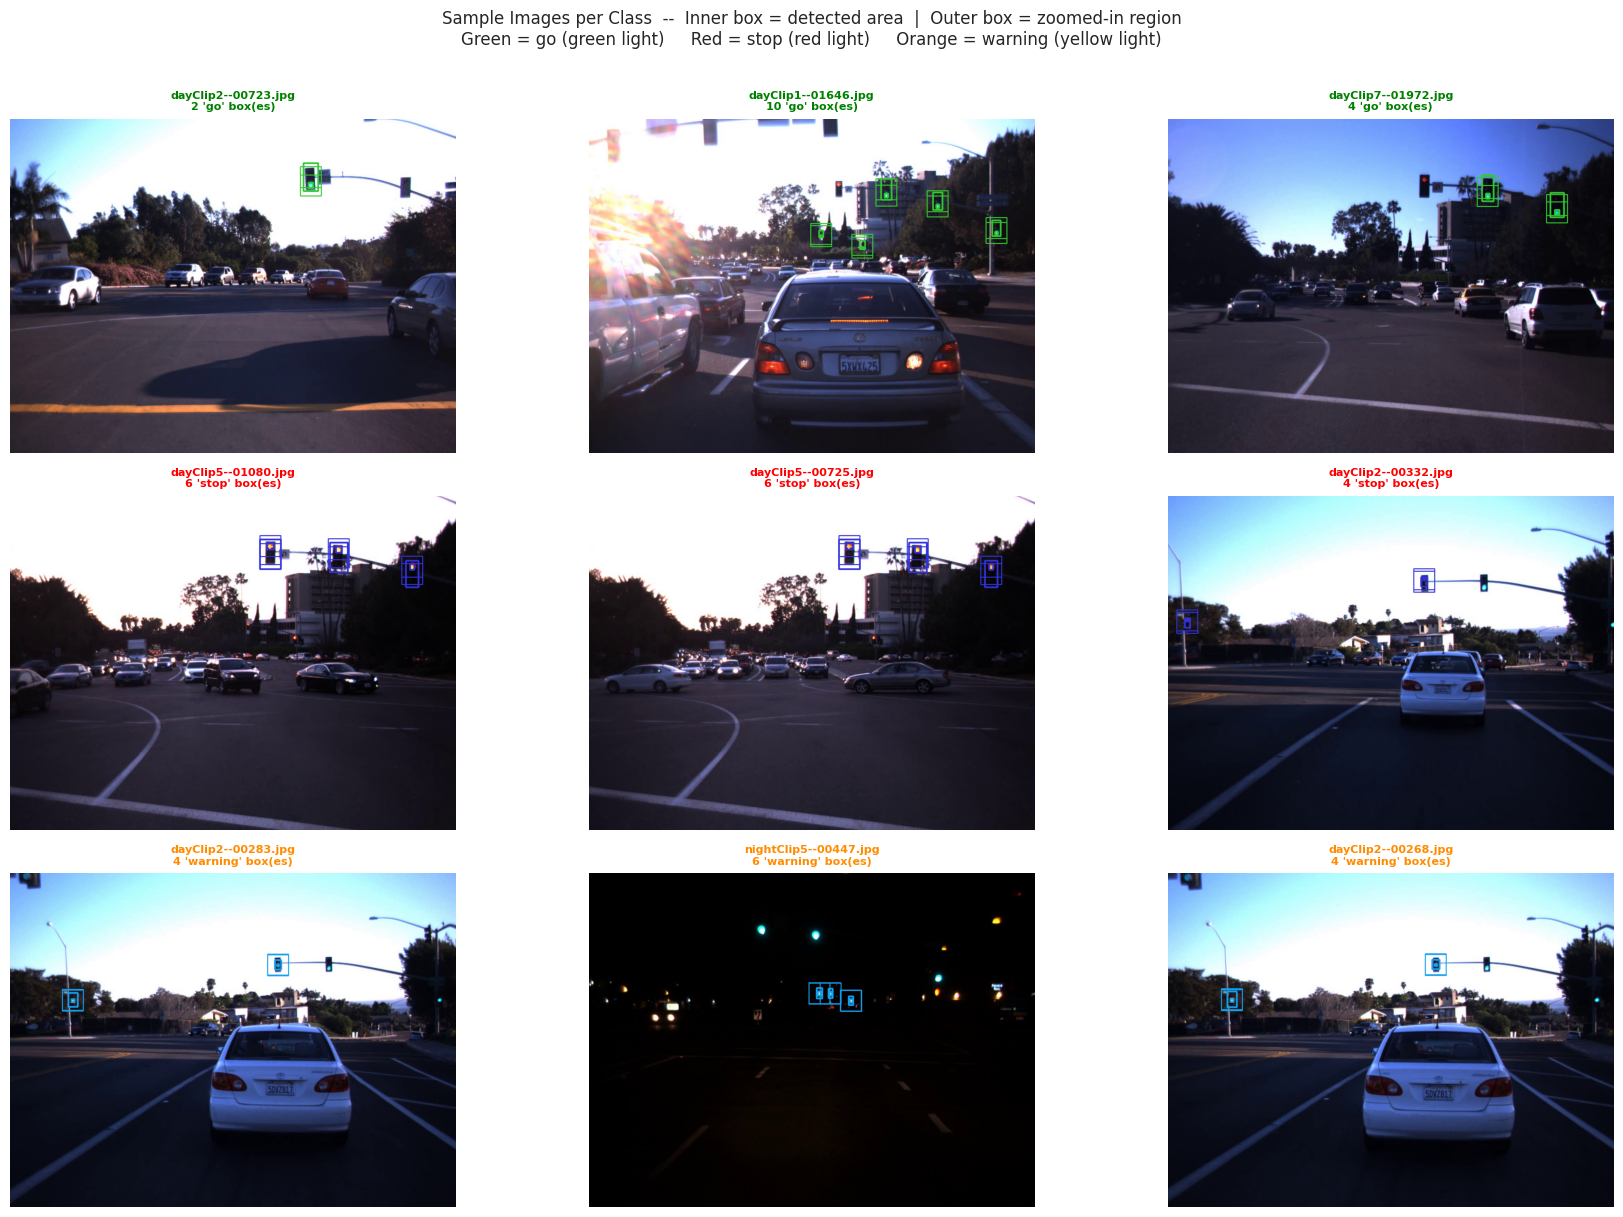
\includegraphics[width=\textwidth]{Images/Chapter2/class_samples.png}
    \end{center}
    \caption{Representative sample images for each class: go (green), stop (red), and warning (orange), with annotated bounding boxes.}
    \label{fig:class_samples}
\end{figure}

\section{Class Mapping}

The 14 original class labels were consolidated into three semantic classes to reduce task complexity and reflect the actual traffic signal states that a driver assistance system must respond to. Table~\ref{tb:classmap} presents the complete mapping.

\begin{table}[htbp]
\caption{Mapping of 14 original LISA class labels to three semantic classes.}
\label{tb:classmap}
\centering
\small
\begin{tabular}{>{\raggedright\arraybackslash}p{0.56\textwidth} l c}
\toprule
\textbf{Original Class Label} & \textbf{Semantic Class} & \textbf{Class ID} \\
\midrule
go & go & 0 \\
go traffic light & go & 0 \\
go left & go & 0 \\
go left traffic light & go & 0 \\
go forward & go & 0 \\
go forward traffic light & go & 0 \\
stop & stop & 1 \\
stop traffic light & stop & 1 \\
stop left & stop & 1 \\
stop left traffic light & stop & 1 \\
warning & warning & 2 \\
warning traffic light & warning & 2 \\
warning left & warning & 2 \\
warning left traffic light & warning & 2 \\
\bottomrule
\end{tabular}
\end{table}

It should be noted that the classes ``go forward'' and ``go forward traffic light'' appear exclusively in the test annotation split and are handled correctly during test evaluation by the same mapping applied to the training data.

\section{Label Format Conversion}

The YOLOv8 training framework requires labels in a specific normalised text format. For each bounding box, the label file contains the class identifier followed by four normalised spatial parameters: centre x-coordinate, centre y-coordinate, width, and height --- all expressed as fractions of the image dimensions. The conversion from pixel-space corner coordinates $(x_1, y_1, x_2, y_2)$ to YOLO format follows Equations~\ref{eq:xc} through~\ref{eq:h}.

\begin{equation}
x_c = \frac{x_1 + x_2}{2 \cdot W}
\label{eq:xc}
\end{equation}
\begin{equation}
y_c = \frac{y_1 + y_2}{2 \cdot H}
\label{eq:yc}
\end{equation}
\begin{equation}
w = \frac{x_2 - x_1}{W}
\label{eq:w}
\end{equation}
\begin{equation}
h = \frac{y_2 - y_1}{H}
\label{eq:h}
\end{equation}

where $W$ and $H$ denote the image width and height respectively. All values are clamped to the range $[0, 1]$ to ensure validity. Figure~\ref{fig:label_check} presents a visual verification of the converted labels overlaid on the corresponding images, confirming spatial alignment.

\begin{figure}[ht]
    \begin{center}
        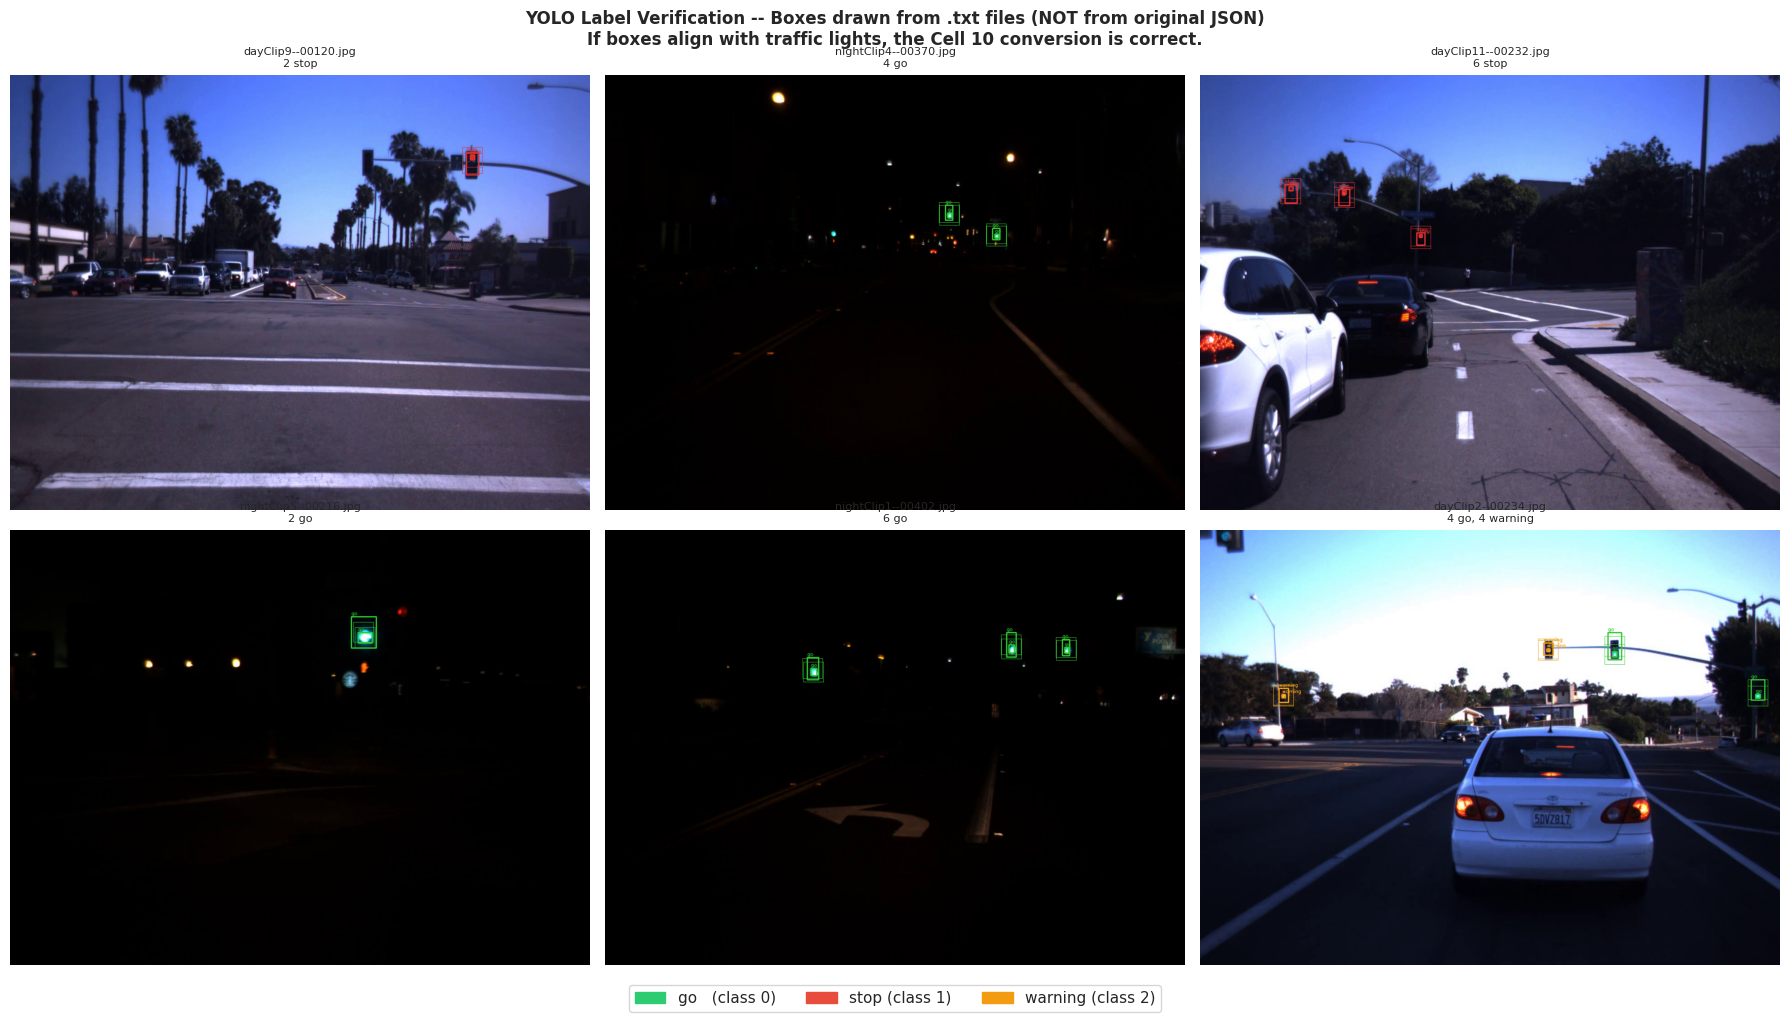
\includegraphics[width=\textwidth]{Images/Chapter2/yolo_label_check.png}
    \end{center}
    \caption[YOLO label conversion verification]{Visual verification of YOLO label conversion: converted bounding boxes overlaid on original images confirming correct spatial alignment.}
    \label{fig:label_check}
\end{figure}

\section{Train/Validation Split Strategy}

The dataset consists of sequential video frames captured in continuous clips (e.g., dayClip1, nightSequence2). A naive random partition at the frame level would place visually near-identical consecutive frames in both the training and validation sets, constituting data leakage that inflates validation accuracy without reflecting real generalisation.

To prevent this, a sequence-level 85/15 split was applied: all frames belonging to a given clip were assigned exclusively to either the training set or the validation set, ensuring that no clip appears in both. This strategy resulted in 17,274 training images and 4,877 validation images. Figure~\ref{fig:split} illustrates the difference between the incorrect frame-level split and the correct sequence-level approach.

\begin{figure}[ht]
    \begin{center}
        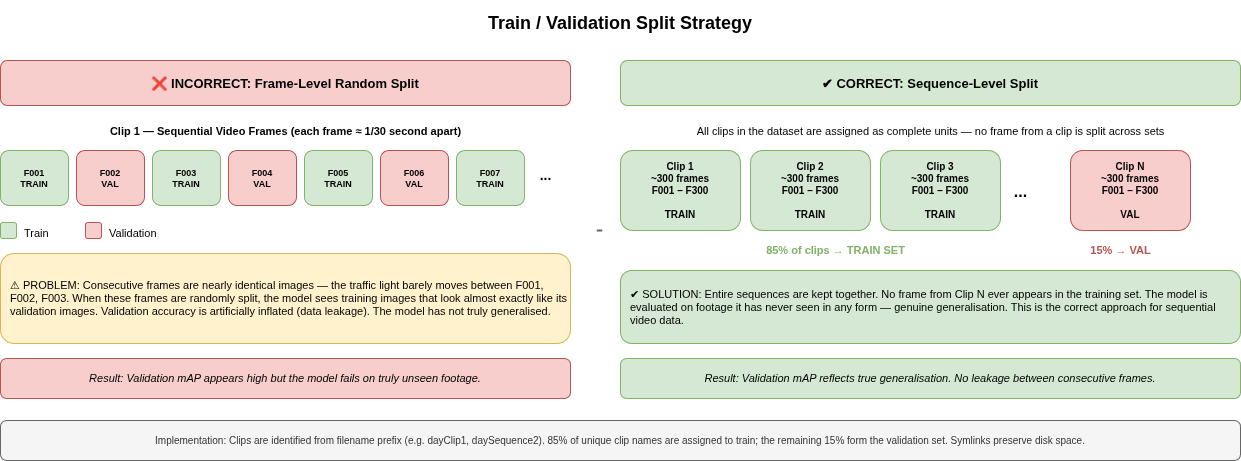
\includegraphics[width=\textwidth]{Images/Diagrams/data_split.png}
    \end{center}
    \caption{Comparison of frame-level split (incorrect, causes data leakage) versus sequence-level split (correct, prevents leakage between train and validation sets).}
    \label{fig:split}
\end{figure}

\section{Class Imbalance Correction}

To address the 19:1 stop-to-warning imbalance identified in Section~\ref{sec:eda-class-dist}, an image-level oversampling strategy was applied to the warning class. Images from clips where warning lights were the dominant annotation were duplicated by creating symbolic file links, targeting a warning class representation of approximately 10\% of the total training images. Symbolic links were used rather than physical file copies to avoid duplicating the dataset storage, which would require an additional $\sim$20\,GB. Following the sequence-level split, the training set comprised 17,274 unique images, and warning-class oversampling was implemented without increasing the storage footprint.

Figure~\ref{fig:sample_boxes} shows a sample of annotated images from the dataset, illustrating the diversity of lighting conditions and scene contexts encountered in training.

\begin{figure}[ht]
    \begin{center}
        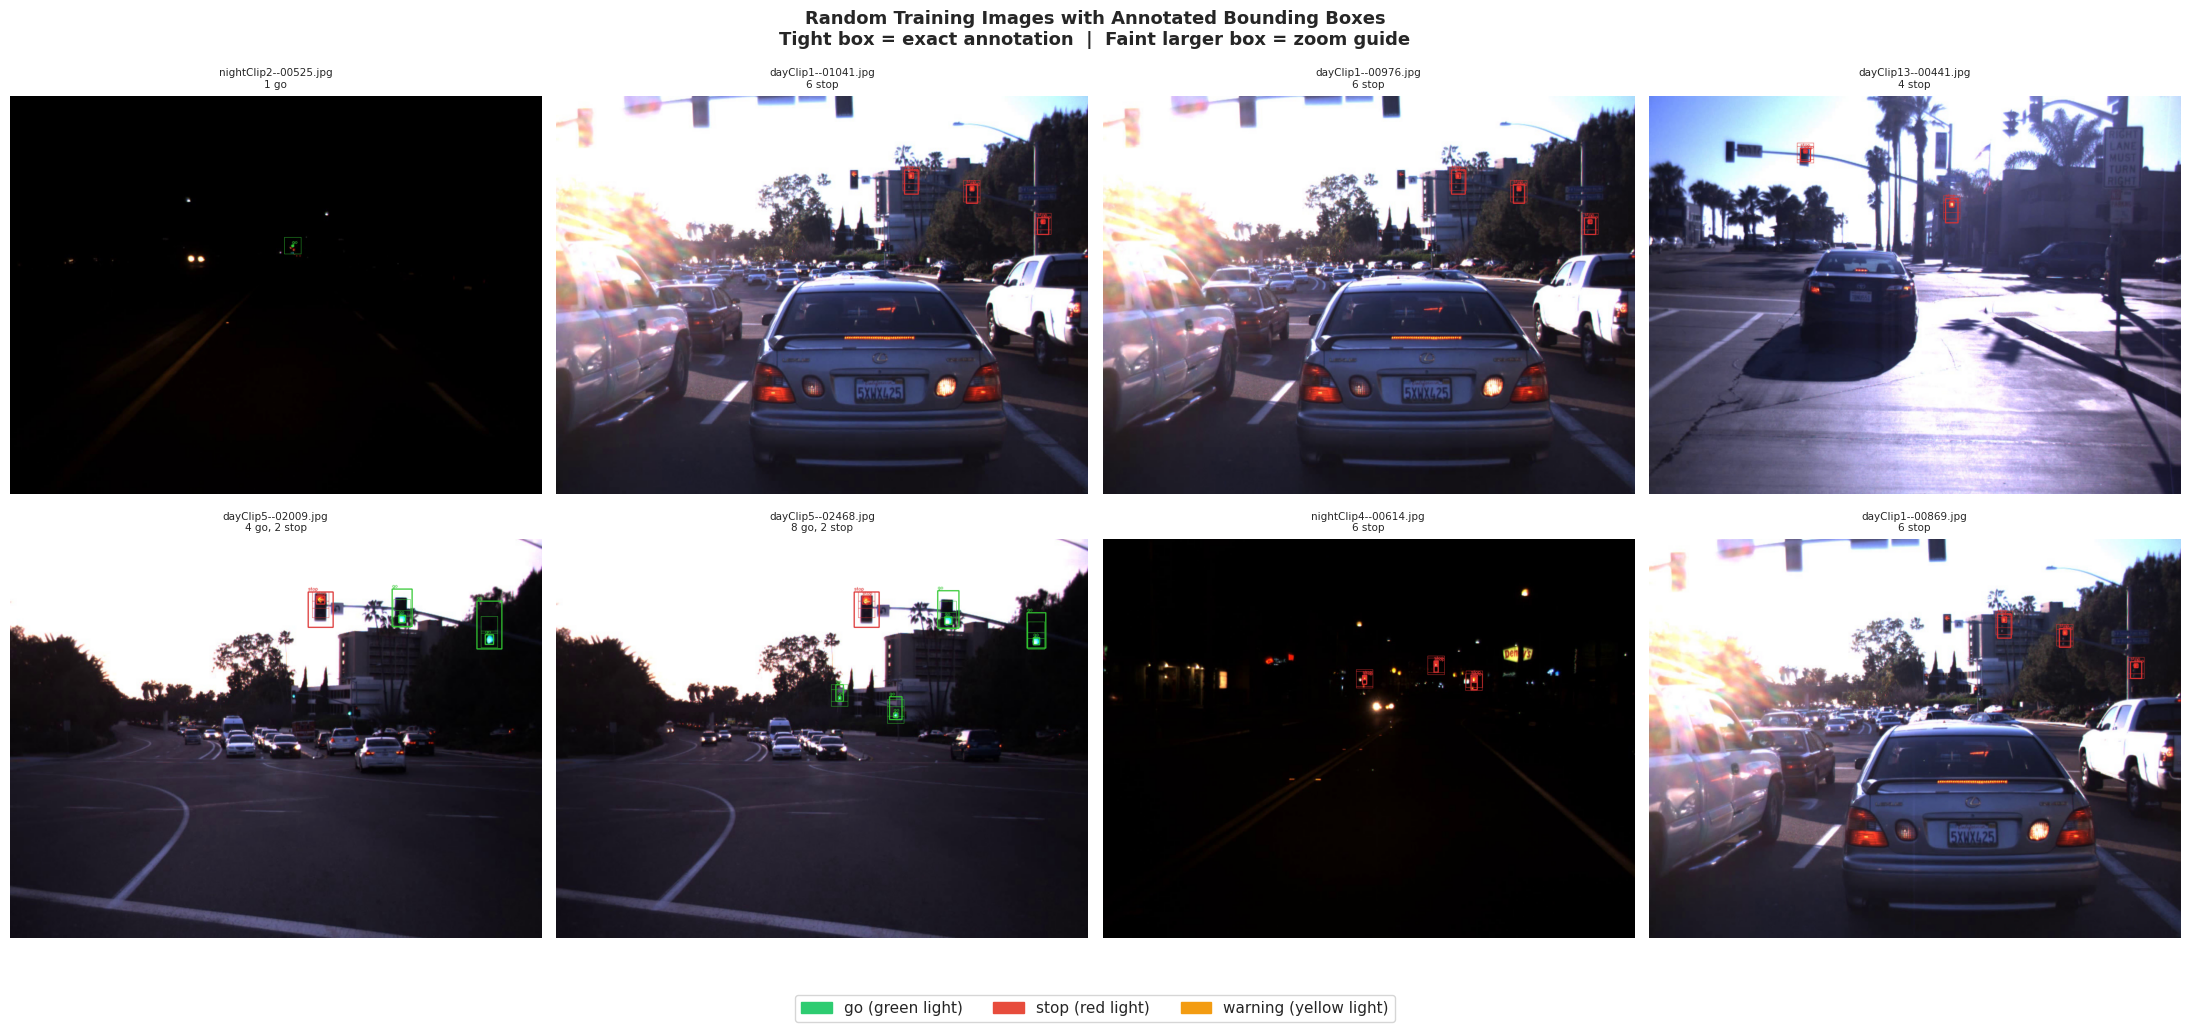
\includegraphics[width=\textwidth]{Images/Chapter2/sample_images_with_boxes.png}
    \end{center}
    \caption{Sample training images with annotated bounding boxes illustrating the diversity of lighting conditions and traffic light appearances in the dataset.}
    \label{fig:sample_boxes}
\end{figure}

%%%%%%%%%%%%%%%%%%%%%%%%%%%%%%%%%%%%%%%%%%%%%%%%%%%%%%%%%%%%%%%%%%%%%%%%%%%%%%%%%%%%%%%%%%%%%%%%%%
%%% END OF FILE
%%%%%%%%%%%%%%%%%%%%%%%%%%%%%%%%%%%%%%%%%%%%%%%%%%%%%%%%%%%%%%%%%%%%%%%%%%%%%%%%%%%%%%%%%%%%%%%%%%
